\chapter{Felhasználói dokumentáció}
\label{ch:user}

\section{Rendszerkövetelmények}

\begin{itemize}
    \item Hardver
    \begin{itemize}
        \item 2 GHz vagy nagyobb órajelű processzor
        \item 2 GB RAM memória
        \item 1 GB lemezterület a RefactorErl, Visual Studio Code, Erlang LS, illetve a bővítmény számára (forráskódok betöltéséhez további tárhely és memória szükséges)
    \end{itemize}
    \item Szoftver
    \begin{itemize}
        \item mac OS El Capitan, Windows 10 vagy Linux operációs rendszer
        \item Telepített RefactorErl elemző eszköz
        \item GraphViz ??? \todo{Graphviz?}
        \item Erlang/OTP 22 vagy újabb \todo{22?}
        \item Visual Studio Code \todo{Version?}
        \item GCC 4.7.2 vagy újabb fordítóprogram
    \end{itemize}
\end{itemize}

\section{Telepítés}
\subsection{Erlang/OTP telepítése}

Mind a RefactorErl futtatásához, mind az Erlang LS futtatéséhoz szükségünk van az Erlang virtuális gép telepítéséhez. Ezt macOS operációs rendszer legegyszerűbben a Homebrew\footnote{\url{https://formulae.brew.sh/formula/erlang\#default}} nevű csomagkezelővel tehetjük meg. Linux és Windows rendszerekhez az Erlang\footnote{\url{"https://www.erlang.org/downloads"}} honlapjáról tájékozódhatunk a telepítő parancsokról, illetve innen tölthetjük le a telepítő állományt is.

\subsection{RefactorErl telepítése}


\subsubsection{[függőségek telepítése]}
\todo{Függősgek, és YAWS}

A RefactorErl egy nyílt forráskódú szoftver, a forráskód letölthető az eszköz honlapjáról.\footnote{https://plc.inf.elte.hu/erlang/refactorerl-releases.html} Miután kicsomagoltuk az ezközt az alábbi parancs segítségével egyszerűen az alábbi parancs segítségével telepíthetjük:

\lstinline{bin/referl -build tool}

\todo{Referl install}
\todo{brew installer?}

\subsection{Visual Studio Code telepítése}
A Visual Studio Code egy cross-platform\footnote{többféle rendszeren képes futni} fejlesztői környezet, ami igen gazdag fejlesztői interfésszel rendelkezik, ami lehetővé tette ezt a fejlesztést is. Megfelelő operációs rendszer kiválasztása után letölthető a termék honlapjáról. \footnote{\url{https://code.visualstudio.com}}

\subsection{RefactorErl Visualiser telepítése}
A Visualiser bővítmény letölthető a bővítmény GitHub oldaláról \footnote{todo\todo{Git oldal}} vagy a mellekélt állományok között is megtalálható a \lstinline{.vsix} kiterjesztésű telepítő fájl. 


\begin{figure}[H]
  \centering
  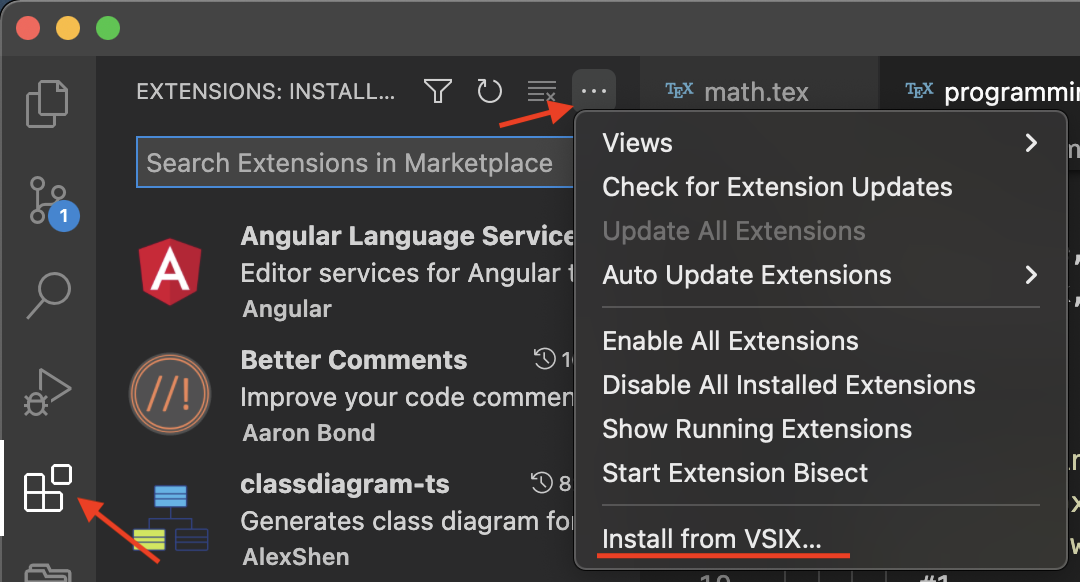
\includegraphics[width=\linewidth]{images/vsix_install.png}
  \caption{Telepítés \lstinline{.vsix} fájlból}
  \label{fig:vsix_install}
\end{figure}
\todo{Ezt highlightolni, illetve ne legyen itt kétszer a kódban}

\subsection{Erlang LS bővített változatának telepítése}
Az Erlang Language Server \textit{eredeti verziója} megtekinthetó a GitHub tárolójában \footnote{todo\todo{LINK A GITHUBHOZ}}, illetve letölthető a Visual Studio Code Marketplace\footnote{todo\todo{LINK AZ ERLANG LS}}-ről 




\section{Erlang LS használata}
\subsection{Első elindításkor szükséges beállítási lehetőségek}
Az első elidulás előtt az Erlang LS konfigurációs fájljában néhány módosítást kell végeznünk, hogy az megfelelően illeszkedjen a RefactorErlhez. A konfigurációs fájl YAML formátumot követ. 
A diagnosztikák futtatásához vegyük fel a \lstinline{refactorerl} elemet az engedélyezettek közé. 

\lstset{caption={RefactorErl diagnosztikák engedélyezése Erlang LS-ben}, label=src:yaml}
\begin{lstlisting}
diagnostics:
  enabled:
    - refactorerl
\end{lstlisting}

Ezzel a beállítással az Erlang LS már futtatni fogja a diagnosztikákat, azonban alapértelmezetten egyetlen diagnosztikai sem fog futni, ezeket manuális allíthatjuk be. Ehhez vegyünk fel egy \lstinline{refactorerl} kulcsot a fájl gyökerébe. Ez alá két \textit{alkulcs} kerülhet:
\begin{itemize}
    \item \lstinline{node}: ide annak az Erlang node\todo{Errre mi a magyar terminológia?}-nak a nevét kell megadni szöveges karakterláncként, ahol a RefactorErl fut. 
    \item \lstinline{diagnostics}: azon diagnosztikák azonosítói, amelyeket futtatni szeretnék listként (felsoroláskén) megadva. A dignosztikák azonosítói szintén szöveges karakterláncok.
\end{itemize}

Példa egy ilyen konfigurációs fájl részletre:

\lstset{caption={RefactorErl konfigurációs példa Erlang LS-ben}, label=src:yaml}
\begin{lstlisting}
diagnostics:
  enabled:
    ...
    - refactorerl

...

refactorerl:
  node: "nodeName@hostName" 		
  diagnostics:
    - "unused_macros"			
    - "unsecure_os_call"
\end{lstlisting}

Az alábbi diagnosztikákból tudunk válogatni jelenleg:

\begin{table}[H]
\centering
\begin{tabular}{|m{0.4\textwidth}|m{0.5\textwidth}|}
 \hline
 Lekérdezés neve & Lekérdezés rövid ismertetése \\ [0.5ex] 
 \hline\hline
 \verb|unsecure_calls| & Az összes lehetséges támadási forma lekérdezése \\ \hline
 \verb|unsecure_interoperability| & Az együttműködési képességből fakadó sebezhetőségek azonosítása. \\ \hline
 \verb|unsecure_concurrency| & A konkurens programozásból eredő hibalehetőségek feltérképezése. \\ \hline
 \verb|unsecure_os_call| & Az ismeretlen helyről származó paraméterekkel meghívott OS szintű utasítások ellenőrzése. \\ \hline
 \verb|unsecure_port_creation| & A portok létrehozásával kapcsolatos sebezhetőségek lekérdezése. \\ \hline
 \verb|unsecure_file_operation| & Az ismeretlen bemenettel meghívott fájlkezeléssel kapcsolatos műveletek lekérése. \\ \hline
 \verb|unstable_call| & Az atomok dinamikus létrehozásával kapcsolatos függvények feltérképezése. \\ \hline
 \verb|nif_calls| & A NIF függvények használatából fakadó sebezhetőségek ellenőrzése. \\ \hline
 \verb|unsecure_port_drivers| & A dinamikusan betölthető könyvtárak használatából fakadó veszélyek azonosítása. \\ \hline
 \verb|decommissioned_crypto| & Az elavultnak számító kriptográfiai műveletek lekérdezése. \\ \hline
 \verb|unsecure_compile_operations| & Az ismeretlen helyről származó programkód fordításának és betöltésének ellenőrzése. \\ \hline
 \verb|unsecure_process_linkage| & A folyamatok nem megfelelő összekapcsolásából adódó sebezhetőségek lekérése. \\ \hline
 \verb|unsecure_prioritization| & A folyamatok prioritásának módosításából fakadó veszélyek ellenőrzése. \\ \hline
 \verb|unsecure_ets_traversal| & Az ETS tábla rögzítés nélküli bejárásának ellenőrzésére szolgáló lekérdezés. \\ \hline
 \verb|unsafe_network| & A hálózati rendszermaggal kapcsolatos műveletek feltérképezése. \\ \hline
 \verb|unsecure_xml_usage| & Az ismeretlen helyről származó xml paraméterek elemzésével kapcsolatos függvények azonosítása. \\ \hline
 \verb|unsecure_communication| & Az elosztott hálózat szereplői között zajló kommunikációs beállítások ellenőrzése. \\ [1ex] 
 \hline
\end{tabular}
\caption{Elérhető diagnosztikai azonosítók listája.}
\label{table:1}
\end{table}


















\subsection{Diagnosztikák használata}
Az Erlang LS a diagnosztikákat az adott szerkesztőben figyelmeztetésként jeleníti meg. Ugyan ez a funckionalitás \textbf{minden ELS-el kompatibilis szerkesztőben meg fog jelenni}, most a példák során a Visual Studio Code szerkesztőre fogunk fókuszálni.



\subsection{Kódakció parancsok kiadása}
\section{Visualiser kiegészítő használata}
\subsection{Elindítása}
\subsection{Egyéni szemantikus lekérdezések}
\subsection{Függőségi gráf rajzolása}
\subsection{Változóhoz kapcsolodó lekérdezések megjelenítése}
\subsection{Dinamikus függvény hívások megjelenítése}
\subsection{Kapcsolat ellenőrzése}
\subsection{Adatbázis szinkronizáció elvégzése}
\subsection{Dinamikus hívás elemzés kezelése}
